\subsubsection{UCA 6 - Tracciamento posizione}%kite level

\begin{figure}[h]
	\centering
	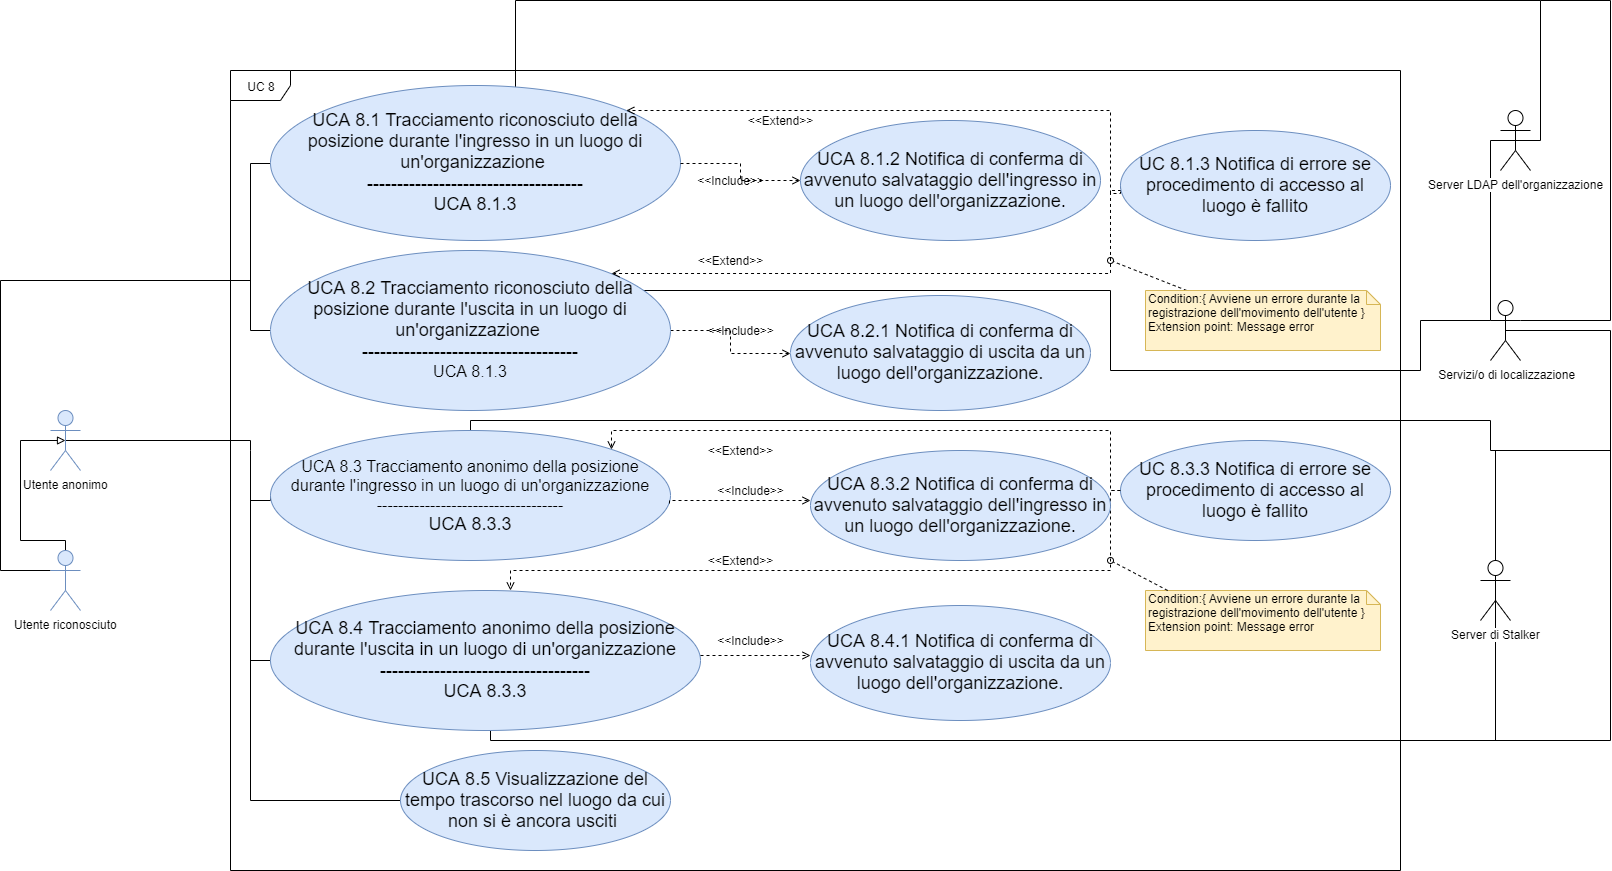
\includegraphics[scale=0.3]{sezioni/UseCase/Immagini/UCA6.png}
	\caption{Tracciamento\ap{G} posizione}
\end{figure}

\begin{itemize}
	\item \textbf{Attori primari:} Utente anonimo, Utente riconosciuto;
	\item \textbf{Attori secondari:} Servizi/o di localizzazione (GPS\ap{G}, rete cellulare);
	\item \textbf{Precondizione:} L'utente autenticato\ap{G} con credenziali Stalker sta per entrare o sta per uscire da un luogo dell'organizzazione che richiede il tracciamento;
	\item \textbf{Postcondizione:} Viene memorizzato dal sistema il timestamp\ap{G} i momenti in cui è avvenuto il tracciamento\ap{G}, dove è avvenuto e il tempo trascorso al suo interno;
	\item \textbf{Scenario principale:} L'utente si trova nei pressi o sta per uscire da un luogo dell'organizzazione che richiede il tracciamento\ap{G}. Viene salvato il timestamp\ap{G} di entrata ed uscita dall'organizzazione e viene salvato il tempo trascorso all'interno dell'organizzazione.
\end{itemize}

\subsubsection{UCA 6.1 - Tracciamento autenticato della posizione durante l'ingresso in un luogo di un'organizzazione}%sea level
\begin{itemize}
	\item \textbf{Attori primari:} Utente riconosciuto;
	\item \textbf{Attori secondari:} Servizi/o di localizzazione (GPS\ap{G}, rete cellulare), server LDAP\ap{G} dell'organizzazione;
	\item \textbf{Precondizione:} L'utente sta per entrare (ovvero si trova nei pressi) in un luogo dell'organizzazione che richiede il tracciamento\ap{G};
	\item \textbf{Postcondizione:} Viene registrato l'ingresso nel luogo dell'organizzazione in una certa data e ora (timestamp\ap{G});
	\item \textbf{Scenario principale:} L'utente, tramite i/il servizio/i di localizzazione, verifica il momento in cui entra al suo interno. Una volta entrato al suo interno, verifica di potersi autenticare correttamente con le credenziali dell'organizzazione [UCA 6.1.2]: se riesce, memorizza nel sistema la data e ora di ingresso nel luogo [UCA 6.1.1]. Infine, viene informato l'utente dell'ingresso riuscito;
	\item \textbf{Scenario alternativo:} Il tentativo di autenticazione\ap{G} presso l'organizzazione o l'invio delle credenziali fallisce. Viene informato l'utente;
	\item \textbf{Estensioni:}
	\begin{enumerate}
		\item UCA 6.1.3 - Notifica di errore se procedimento di memorizzazione dell'accesso al luogo è fallito;
		\item UCA 6.1.4 - Notifica di avvenuta memorizzazione dei dati dell'accesso;
	\end{enumerate}
	\item \textbf{Inclusioni:}
	\begin{enumerate}
		\item UCA 6.1.1 - Invio timestamp\ap{G} relativo all'ingresso/uscita in/da un luogo;
		\item UCA 6.1.2 - Verifica correttezza delle credenziali di accesso all'organizzazione.
	\end{enumerate}
\end{itemize}

% DA 6.1.1 A 6.1.4 RICHIEDONO UN CAMBIO DI NUMERAZIONE PERCHE' NON SONO SOLO RELATIVI A UCA 6.1
\subsubsection{UCA 6.1.1 - Invio timestamp\ap{G} relativo all'ingresso/uscita in/da un luogo}%fish level
\begin{itemize}
	\item \textbf{Attori primari:} Utente riconosciuto, Utente anonimo;
	\item \textbf{Precondizione:} L'utente ha verificato di trovarsi nei pressi di un luogo che richiede il tracciamento\ap{G} autenticato\ap{G};
	\item \textbf{Postcondizione:} Viene registrato il timestamp\ap{G} relativo all'ingresso dell'utente nel luogo dell'organizzazione.
\end{itemize}

\subsubsection{UCA 6.1.2 - Verifica correttezza delle credenziali di accesso all'organizzazione}%fish level
\begin{itemize}
	\item \textbf{Attori primari:} Utente riconosciuto;
	\item \textbf{Attori secondari:} Server \ap{G} dell'organizzazione;
	\item \textbf{Precondizione:} L'utente, in quanto riconosciuto, possiede credenziali per autenticarsi presso l'organizzazione;
	\item \textbf{Postcondizione:} Viene verificata o meno la validità delle credenziali fornite: esse sono valide se la verifica va a buon fine.
\end{itemize}

\subsubsection{UCA 6.1.3 - Notifica di errore se procedimento di memorizzazione dell'accesso al luogo è fallito}%fish level
\begin{itemize}
	\item \textbf{Attori primari:} Utente riconosciuto, Utente anonimo;
	\item \textbf{Precondizione:} Avviene un errore durante la registrazione dell'accesso dell'utente;
	\item \textbf{Postcondizione:} Viene notificato l'errore all'utente.
\end{itemize}

\subsubsection{UCA 6.1.4 - Notifica di avvenuta memorizzazione dei dati dell'accesso}%fish level
\begin{itemize}
	\item \textbf{Attori primari:} Utente riconosciuto, Utente anonimo;
	\item \textbf{Precondizione:} Il processo di memorizzazione dei dati dell'accesso nel sistema è avvenuto correttamente;
	\item \textbf{Postcondizione:} Viene notificato l'utente dell'avvenuto salvataggio.
\end{itemize}

\subsubsection{UCA 6.2 - Tracciamento riconosciuto della posizione durante l'uscita in un luogo di un'organizzazione}%sea level
\begin{itemize}
	\item \textbf{Attori primari:} Utente riconosciuto;
	\item \textbf{Attori secondari:} Servizi/o di localizzazione (GPS\ap{G}, rete cellulare), server LDAP\ap{G} dell'organizzazione;
	\item \textbf{Precondizione:} L'utente sta per uscire da un luogo dell'organizzazione che richiede il tracciamento\ap{G};
	\item \textbf{Postcondizione:} Viene registrato l'uscita dal luogo dell'organizzazione in una certa data e ora (timestamp\ap{G});
	\item \textbf{Scenario principale:} L'utente, quando verifica tramite i/il servizi/o di localizzazione che sta per uscire da un luogo dell'organizzazione, verifica il momento in cui avviene l'uscita. Quando esce, verifica di potersi autenticare correttamente con le credenziali dell'organizzazione [UCA 6.1.2]: se riesce, memorizza nel sistema la data e ora di uscita dal luogo [UCA 6.1.1]. Infine, viene informato l'utente dell'uscita riuscita. La combinazione di ingresso effettuato in precedenza e dell'uscita effettuata formano un accesso, ora ritrovabile in Storico accessi [UCA 5];
	\item \textbf{Scenario alternativo:} Il tentativo di autenticazione\ap{G} presso l'organizzazione o l'invio delle credenziali fallisce. Viene informato l'utente;
	\item \textbf{Estensioni:}
	\begin{enumerate}
		\item UCA 6.2.3 - Notifica di errore se procedimento di memorizzazione dell'accesso al luogo è fallito;
		\item UCA 6.2.4 - Notifica di avvenuta memorizzazione dei dati dell'accesso;
	\end{enumerate}
	\item \textbf{Inclusioni:}
	\begin{enumerate}
		\item UCA 6.2.1 - Invio timestamp\ap{G} relativo all'ingresso/uscita in/da un luogo;
		\item UCA 6.2.2 - Verifica correttezza delle credenziali di accesso all'organizzazione.
	\end{enumerate}
\end{itemize}

\subsubsection{UCA 6.3 - Tracciamento anonimo della posizione durante l'ingresso in un luogo di un'organizzazione}%sea level
\begin{itemize}
	\item \textbf{Attori primari:} Utente anonimo;
	\item \textbf{Attori secondari:} Servizi/o di localizzazione (GPS\ap{G}, rete cellulare);
	\item \textbf{Precondizione:} L'utente sta per entrare (ovvero si trova nei pressi) in un luogo dell'organizzazione che richiede il tracciamento\ap{G};
	\item \textbf{Postcondizione:} Viene registrato l'ingresso nel luogo dell'organizzazione in una certa data e ora (timestamp\ap{G});
	\item \textbf{Scenario principale:} L'utente, tramite i/il servizio/i di localizzazione, verifica il momento in cui entra al suo interno. Quando entra al suo interno memorizza nel sistema la data e ora di ingresso nel luogo [UCA 6.1.1]. Infine, viene informato l'utente dell'ingresso riuscito;
	\item \textbf{Scenario alternativo:} Il tentativo di invio delle credenziali fallisce. Viene informato l'utente.
	\item \textbf{Estensioni:}
	\begin{enumerate}
		\item UCA 6.3.3 - Notifica di errore se procedimento di memorizzazione dell'accesso al luogo è fallito;
		\item UCA 6.3.4 - Notifica di avvenuta memorizzazione dei dati dell'accesso;
	\end{enumerate}
	\item \textbf{Inclusioni:}
	\begin{enumerate}
		\item UCA 6.3.1 - Invio timestamp\ap{G} relativo all'ingresso/uscita in/da un luogo.
	\end{enumerate}
\end{itemize}

\subsubsection{UCA 6.4 - Tracciamento anonimo della posizione durante l'uscita in un luogo di un'organizzazione} %sea level
\begin{itemize}
	\item \textbf{Attori primari:} Utente anonimo;
	\item \textbf{Attori secondari:} Servizi/o di localizzazione (GPS\ap{G}, rete cellulare);
	\item \textbf{Precondizione:} L'utente sta per uscire da un luogo dell'organizzazione che richiede il tracciamento\ap{G};
	\item \textbf{Postcondizione:} Viene registrato l'uscita dal luogo dell'organizzazione in una certa data e ora (timestamp\ap{G});
	\item \textbf{Scenario principale:} L'utente, quando verifica tramite i/il servizi/o di localizzazione che sta per uscire da un luogo dell'organizzazione, verifica il momento in cui avviene l'uscita. Quando esce, memorizza nel sistema la data e ora di uscita dal luogo [UCA 6.1.1]. Infine, viene informato l'utente dell'uscita riuscita. La combinazione di ingresso effettuato in precedenza e dell'uscita effettuata formano un accesso, ora ritrovabile in Storico accessi [UCA 5];
	\item \textbf{Scenario alternativo:} Il tentativo di invio delle credenziali fallisce. Viene informato l'utente.
	\item \textbf{Estensioni:}
	\begin{enumerate}
		\item UCA 6.4.3 - Notifica di errore se procedimento di memorizzazione dell'accesso al luogo è fallito;
		\item UCA 6.4.4 - Notifica di avvenuta memorizzazione dei dati dell'accesso;
	\end{enumerate}
	\item \textbf{Inclusioni:}
	\begin{enumerate}
		\item UCA 6.4.1 - Invio timestamp\ap{G} relativo all'ingresso/uscita in/da un luogo.
	\end{enumerate}
\end{itemize}